% Author Alfredo Sánchez Alberca (asalber@ceu.es)

\section{Charts}
\begin{enumerate}[leftmargin=*,resume]
\item Open the Excel workbook created in exercise~\ref{ex-sales-forecast} and create an appropriate chart to describe
the sales and expenses forecast evolution. 

\item Open the Excel workbook created in exercise~\ref{ex-quarter-payroll} an create a chart like the one below. 
\begin{center}
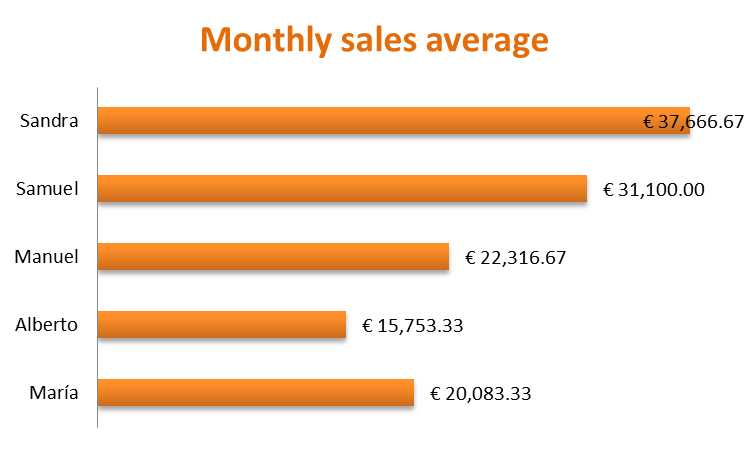
\includegraphics[scale=0.8]{img/quarter-payroll}
\end{center}

\item Open the Excel workbook created in exercise~\ref{ex-basic-formatting} and create a chart like the one below.
\begin{center}
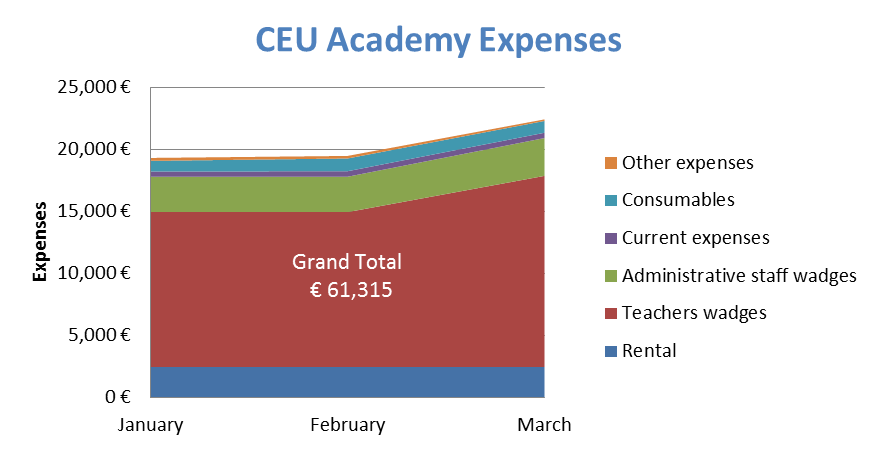
\includegraphics[scale=0.8]{img/basic-formatting}
\end{center}

\item Open the Excel workbook created in exercise~\ref{ex-income-quarters} and create a chart appropriate to describe
the part of the annual income that correspond to fixed commissions, variable commissions, taxes and profit after taxes
(PAT).

\item Open the Excel workbook created in exercise~\ref{ex-car-dealerships} and create a chart like the one below.
\begin{center}
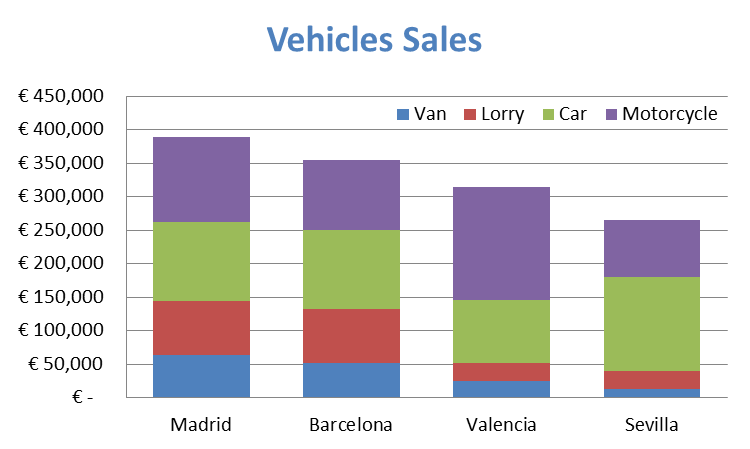
\includegraphics[scale=0.8]{img/car-dealerships}
\end{center}

\item Open the Excel workbook created in exercise~\ref{ex-lemonade} and create a chart like the one below.
\begin{center}
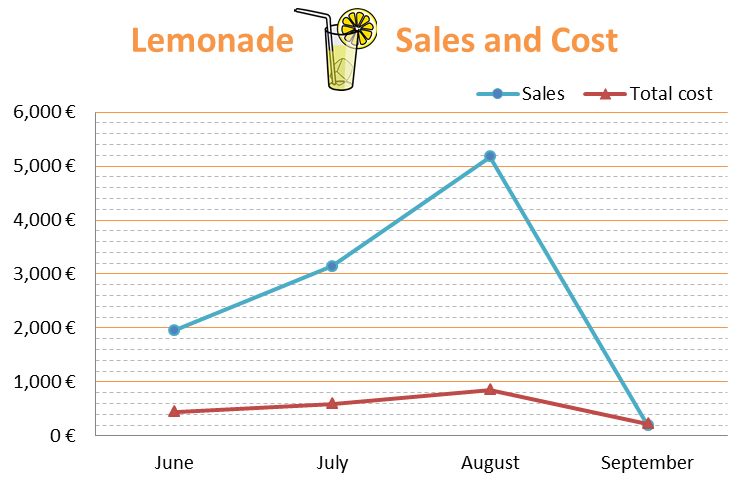
\includegraphics[scale=0.8]{img/lemonade}
\end{center}

\item Open the Excel workbook created in exercise~\ref{ex-salary-sellers} and create a chart like the one below.
\begin{center}
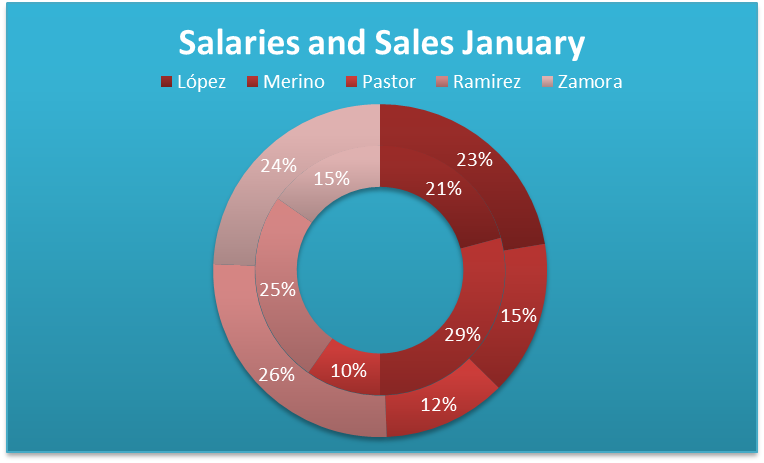
\includegraphics[scale=0.8]{img/salary-sellers}
\end{center}

\item Open the Excel workbook create in exercise~\ref{ex-laboratory-suppliers} and create a chart like the one below. 
\begin{center}
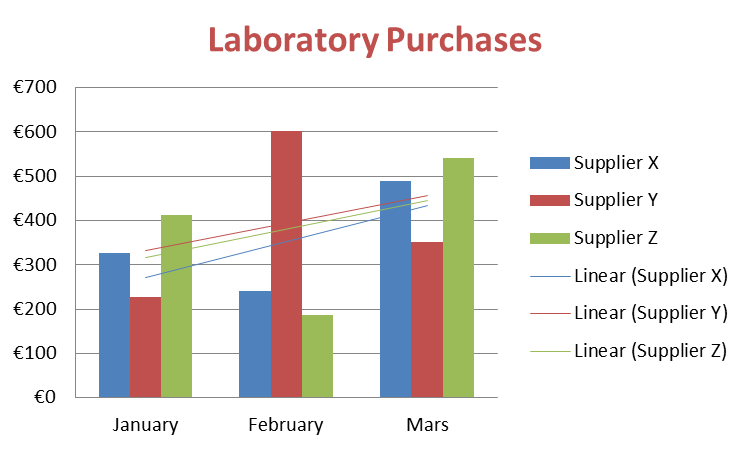
\includegraphics[scale=0.8]{img/laboratory-suppliers}
\end{center}

\item The table below shows the income and savings of 8 families in one month.
\begin{center}
\begin{tabular}{lrrrrrrrr}
\toprule
Income(€)  & 1240 & 1480 & 900 & 1120 & 2030 & 1570 & 1680 & 1300\\
Savings(€) &  220 &  450 & 110 &  375 &  560 &  480 &  525 &  290\\
\bottomrule
\end{tabular}
\end{center}
Create an appropriate chart to show the relation between income and savings. 
\end{enumerate}